\graphicspath{{./}{./figures/}{./figures/neural/}}

\chapter{Neural Synthesis}

\section{Introduction}
Music producers and sound-effect artists require the frequent use of audio samples, for example to simulate a snare drum hit or a gunshot sound. The process of arduously searching through multi-gigabyte sound libraries for the right sound is extremely time-consuming; and its alternative, of creating a brand new sound using audio synthesizers, requires a formidable technical background. To compound this difficulty, in a track or action scene containing hundreds of snare drum hits or gunshots, the process of using the same (or same few) samples repeatedly can lead to a canned effect. What is required is a method for simultaneously trimming down the size of a library while simultaneously (and in some sense paradoxically) increasing sound variability.

In this work, we use Generative Adversarial Networks (GANs) \cite{goodfellow2014generative} to generate new instrumental audio from a dataset of existing material. GANs have the potential to be used to generate new sounds on the fly. This would dramatically alleviate both the problem of having to pore through giant sound libraries, and the problem with having to only use one sample repeatedly. In addition, the explosion of new sounds which could potentially be produced by GANs would vastly reduce recording costs by designers of sound libraries.

This research avenue is to a certain degree untapped: GANs have been successfully applied to the generation and manipulation of images, however, relatively little work has been focused on the audio domain. Research related to the specific work proposed here was presented by \cite{donahue2018adversarial}  and \cite{engel2018gansynth}.

Through the work in our project, we implemented a GAN following the approach of \cite{donahue2018adversarial}, and trained it using instrumental audio samples from the freely available NSynth dataset\footnote{\url{https://magenta.tensorflow.org/datasets/nsynth}}, published by \cite{nsynth2017} from Google's Magenta research lab. The NSynth dataset contains over 300k four second long audio samples of labelled musical instruments, including flute, brass, string, and other instrument sounds. We explored several variations to the baseline model proposed by \cite{donahue2018adversarial}, including a perceptually motivated model using spectrograms. Our results show that the time-domain based model performed the best for our instrumental synthesis task, and one of the major findings of our project show that significant improvements were made by adding dropout to generator model.

\section{Problem Definition}
The specific problem that was being tackled was the generation of one second of audio in the style of a specific, solo musical instrument. The focus of our initial experiments was to train a GAN to generate one second of a flute sound at a specific pitch. We followed the general approach of \cite{donahue2018adversarial} in implementing a WaveGAN, a GAN the produce time-domain audio signals. Among the features implemented in the WaveGAN are a DCGAN architecture, a Wasserstein loss function, phase shuffling to make training easier for the generator and inception and nearest-neighbor scores for evaluation. Of these features, the only one we had no time to implement was the inception score. 

Additionally, we developed an idea on our own for a variation on the WaveGan model that uses the Mel-Spectrogram. This reframes the audio generation problem back into the image generation domain by using a time series of mel-scale frequency bands to create a spectrogram image. Donahue et al. experimented with a similar approach using the Short-time Fourier Transform (STFT). The STFT is a linear frequency audio representation. However, humans perceive frequency in a logarithmic scale. Mel-Spectrograms represent audio in the frequency domain using the mel-frequency scale, which is a logarithmic based scale based on human auditory perception. While MFCCs are typically not invertible, there exist approximations allowing for transform to the time-domain, with which we experimented and compared results to the time-domain based GAN that we also developed. This approach is somewhat analogous to the SpecGAN implemented by Donahue et al.

Additionally, we attempted some architecture variations, in an attempt to eliminate checkerboard artifacts and improve overall model training. Based our these findings we trained GANs using a selection of other instruments.

\section{Related Work, Background Information}

The concept of Generative Adversarial Nets was introduced in 2014 by \cite{goodfellow2014generative}. A tremendous amount of research has been devoted to the topic of improving GANs. An architecture which has been shown to work well in practice for generating images is the Deep Convolution Neural Network (\cite{radford2015unsupervised}).

One problematic feature of the DCGAN, however, is its propensity for generating checkerboard artifacts, as visible in Figure \ref{checkerboard}. These are believed to be an effect of the transpose-convolution layers in the DCGAN generator. One possible solution, proposed by \cite{Odena2016DeconvolutionAC} is the use of resize or upsampling layers.

\begin{figure}
\centering
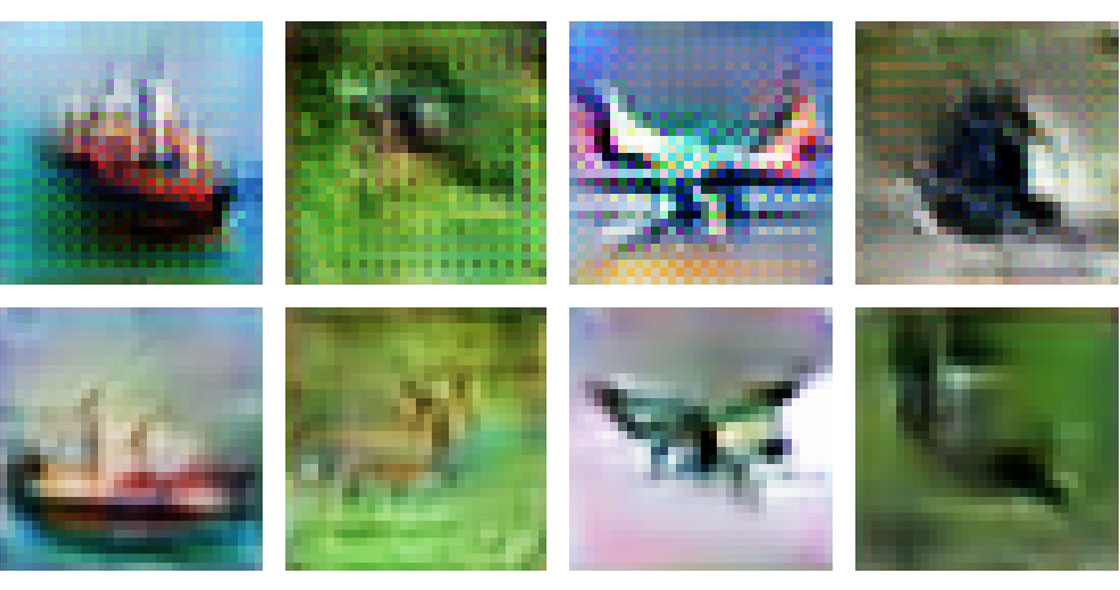
\includegraphics[width=0.8\textwidth]{checkerboard.jpg}
\caption{We see examples of the checkerboard effect commonly associated with GANs which use the transpose convolution. Credit: \cite{Odena2016DeconvolutionAC}.}
\end{figure}\label{checkerboard}

An important technical advancement in the theory of GANs was to relax the topology on the probability distributions from the strong to weak-* topologies (for more information, see Appendix A). This gave rise to the Wasserstein GAN, as proposed by \cite{arjovsky2017wasserstein}. The Lipschitz constraint was naively implemented in the original by weight clipping. Later, \cite{gulrajani2017improved} considered a more sophisticated solution, the WGAN-GP (Wasserstein GAN - Gradient Penalty), which relied on insights from the field of optimal transport (see for example \cite{villani_2009}).

The foregoing technology was developed to solve the problem of image generation. Donahue et al. (\cite{donahue2018adversarial}) have applied the WGAN-GP to the problem of audio generation. Their application was done along two different lines. The first, and most obvious method was to apply standard GAN image generation techniques to audio spectrograms (the SpecGAN). The second method was to slightly reframe the DCGAN architecture to accommodate 1-dimensional time series data (waveforms) instead of 2-dimensional images (the WaveGAN). They found slightly better success in the latter approach.

\section{Methods}
We first attempted to recreate the baseline WaveGAN algorithm proposed by \cite{donahue2018adversarial}, which was a simple modification to DCGAN. The DCGAN model, which generated images in the style of the MNIST dataset, was developed first, and then modified to accommodate one second long audio samples instead of images. This modification involved flattening the DCGAN layers to support one-dimensional signals instead of two-dimensional images. The original DCGAN model supported 64x64 pixel images, which corresponds to a 4096 length signal when flattened. To support audio signals one second long at a sampling rate of 16kHz, an additional convolution layer was added to bring to the final output of the generator up to 16384. The discriminator model from DCGAN was modified in a similar manner. Further details on this architecture are provided in Appendix B.

\subsection{WGAN-GP}
Building on this baseline DCGAN architecture, the WGAN-GP was implemented by modifying the loss functions and implementing a gradient penalty that is added to the discriminator loss. The baseline DCGAN model was trained using the approach proposed by \cite{goodfellow2014generative}, which seeks to solve the following dual minimization problem:
\begin{equation*}\label{eqn:goodfellow_minimization}
    \min_{G}\left(\max_{D}\left(\sum_{x\text{ real}}\log(D(x))-\sum_{z\text{ latent}}\log(D(G(z)))\right)\right)
\end{equation*}

where $N$ samples are taken i.i.d. from the space of real waveforms, and the latent space, respectively. The generator $G$ and the discriminator $D$ are allowed to be arbitrary neural networks, in this case the modified DCGAN networks. Note that this is not precisely the form of loss derived in Appendix A; it has been slightly modified to avoid vanishing gradients.

In the case of the WGAN, the loss is modified to:
\begin{equation*}
    \min_{G}\left(\max_{D}\left(\sum_{x\text{ real}}D(x)-\sum_{z\text{ latent}}D(G(z))\right)\right)
\end{equation*}
where now $D$ is required to have gradient norm $\leq 1$. This condition is achieved by applying a gradient penalty on convex combinations pairs of points from the real, and generated datasets.

\subsection{Architecture Variations}\label{sec:variation}
\subsubsection{Mitigating Checkerboard Artifacts}
A number of variations to the the model architecture were explored in attempt to improve the quality of audio generated. The checkerboard artifacts identified by \cite{Odena2016DeconvolutionAC} present additional challenges in the realm of audio signals compared to images. \cite{donahue2018adversarial} note that in the case of images, the discriminator might be able to use these artifacts as a way of identifying fakes images, whereas in audio signals repeating patterns are common in pitched signals which could introduce additional challenges for the discriminator in distinguishing between intentional repetitions and artifacts. Finding ways to mitigate these artifacts is beneficial as they result in unpleasant distortions in the final audio signals.

The first approach that we applied to remedy this issue was to apply resizing layers, which was suggested by \cite{Odena2016DeconvolutionAC}. The resizing layers precede the convolution layers in the generator and take over the role of upsampling the signal, which was previously handled using transpose operations within the convolution. One the of the effects that these resizing layers have is mitigating the effect of aliasing that can occur during upsampling using transpose convoluation layers. Four different methods for resizing were tested: basic upsampling, nearest neighbour interpolation, linear interpolation, and cubic interpolation.

The second approach that we explored to mitigate the adverse effect checkerboard artifacts on training was phase shuffling, proposed by \cite{donahue2018adversarial}. Phase shuffling is applied after each convolution layer in the discriminator and applies a small random time shift by $-N$ to $N$ samples to the signal, where $N$ is a hyperparameter set to control the amount of shifting applied. This process makes the discriminator's job more challenging by forcing it to handle phase invariance.

\subsubsection{Batch Normalization}
Batch normalization can be applied after each convolution layer to normalize results prior to the next layer. This was applied to all layers in both the generator and discriminator in the original DCGAN model. Removing batch normalization in the discriminator was a necessity due to the addition of the gradient penalty in the WGAN-GP, as described by \cite{gulrajani2017improved}. In the case of the generator, \cite{donahue2018adversarial} experimented with also removing batch normalization from the generator. We also experiment with removing batch normalization from the generator model.

\subsubsection{Dropout}
Dropout is a regularization method used in deep learning networks to combat overfitting \cite{srivastava2014dropout}. When using dropout, a percentage of nodes from an output layer are randomly left out, which has been found to improve training. A dropout of 30\% was included in the discriminator from the original DCGAN model and was left in throughout experiments. We experimented with adding 50\% dropout to the generator model.

\subsubsection{Kernel Size}
Adjusting the kernel size in the discriminator affects to number of parameters in the model and therefore the capacity of the model. The original image DCGAN model used a kernel size of (5x5) which translates to a kernel size of 25 in the audio DCGAN discriminator. To reduce the complexity of the discriminator in our initial experiments we used a smaller kernel size of 5, which allowed for quicker training time for the initial model variations. Later experiments modified this kernel size and experimented with increasing the size up to 15 and 25. The kernel size in the generator was kept at 25 throughout all experiments.

\subsection{MelGAN}\label{sec:methods_melgan}
Using a spectrogram representation of audio reframes the audio GAN problem back into the image domain. \cite{donahue2018adversarial} experimented with this approach with their proposed SpecGAN by producing spectrogram images of size (128x128) using the Short-Time Fourier Transform (STFT). One issue with the STFT is that it produces linear-spaced frequency-bins and humans perceive pitch and frequency on a logarithmic scale. The mel-frequency scale is a perceptually informed scaling based on human hearing and techniques exist to map the results from the STFT onto this frequency scale \cite{stevens1940relation}. One issue with using spectrograms for audio generation is that they are not typically invertible due the loss of phase information during spectrogram creation. In order to perform signal reconstruction in this case, phase can be estimated using the Griffin-Lim algorithm \cite{griffin1984signal}, which is the approach we took here.

%\begin{figure}
%\centering
%\includegraphics[width=0.48\textwidth]{MelSpectroGram %transform.png}
%\caption{Conversion of an audio time series signal to a mel-spectrogram. Mel-spectrogram is produced using a Short-Time Fourier Transform with size 2056, hop length of 128. Resulting linear frequency bins are mapped to 128 mel-frequency bins. The x-axis of the mel-spectrogram represents time and the y-axis frequency in the mel-scale, the magnitude of each value in the mel-spectrogram represents the energy at that frequency and time.}
%\end{figure}\label{fig:melspectrogram}

To explore the benefit of using a perceptually motivated spectrogram for audio generation, we experiment with using mel-spectrograms in combination with the WGAN-GP, we call the resulting model MelGAN. The time-series training data was converted to the time-frequency domain using the STFT with an FFT of size 2056 and a hop-length of 128 samples. The resulting linear frequency bins were then mapped to 128 mel-frequency bins. The amplitude was then converted to a logarithmic scale, which is a more perceptual relevant measurement of amplitude, and then scaled to a range between 0 and 1. This resulted in a set of mel-spectrogram images of size (128x128). The flattened DCGAN architecture was converted back to a model that could handle images. %Figure \ref{fig:melspectrogram} shows an example of a time-domain audio signal and its resulting mel-spectrogram.


\section{Experiments}
All experiments were conducted using the NSynth dataset \cite{nsynth2017}. Initial experiments comparing the DCGAN to the WGAN-GP were conducted using all flute samples from the NSynth dataset, which resulted in 8773 unique samples. All audio had a sampling rate of 16kHz and was trimmed to a length of 16,384, just over one second long. The amplitude of the dataset was normalized so the absolute value of the maximum sample was 1. Both DCGAN and WGAN-GP models were trained for 200 epochs using batch sizes of 64.

The results, showcased in Figure \ref{dcgan_wpgan}, were fairly dramatic, showing the improvement that the WGAN-GP approach provided in supporting the generator to learn. Armed with this empirical evidence as well as the mathematical justification in Appendix A, we proceeded to use the WGAN-GP thereafter. The following sections outline the experiments that were conducted in attempt to improve upon the baseline model trained using the WGAN-GP approach, as well as experiments in training the model on a range of different instrument types.

\begin{figure}
\centering
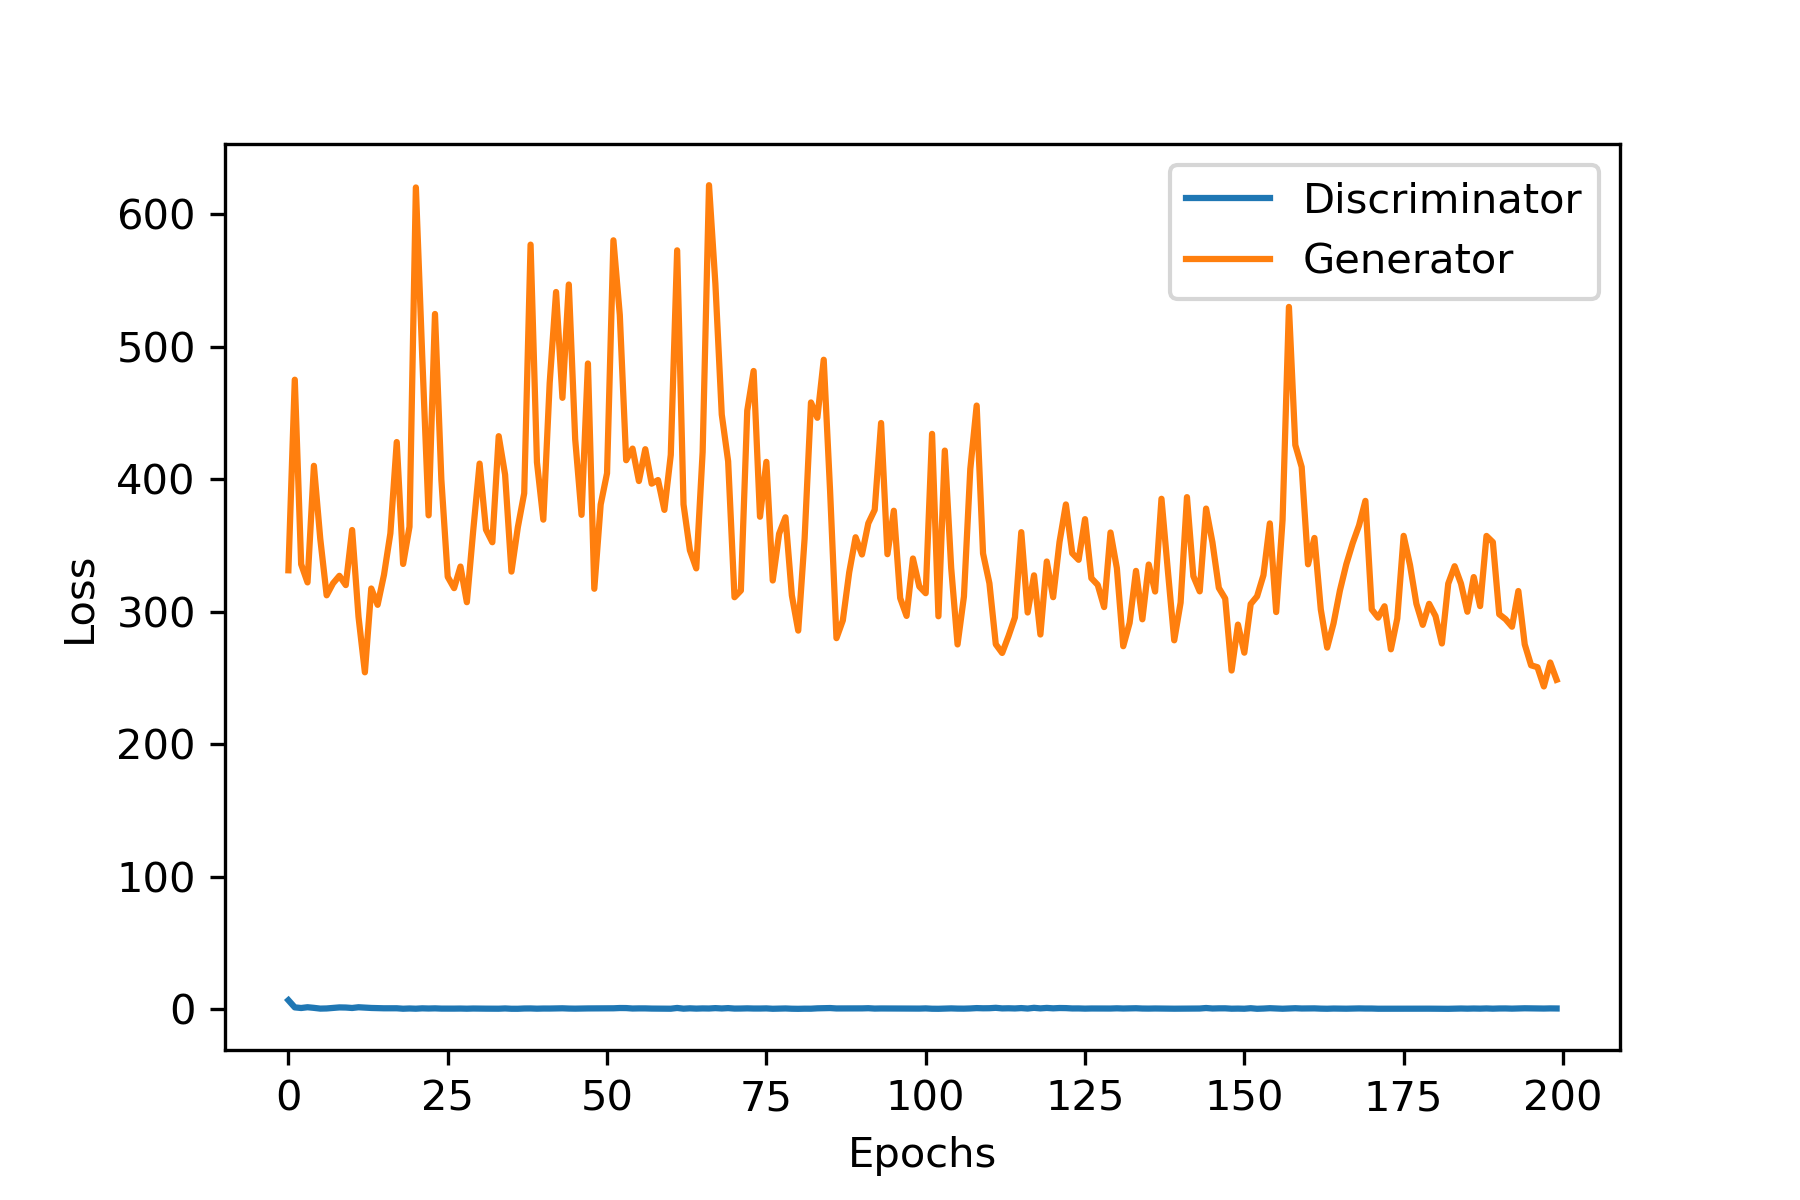
\includegraphics[width=0.48\textwidth]{0725_flute_dcgan_loss.png}
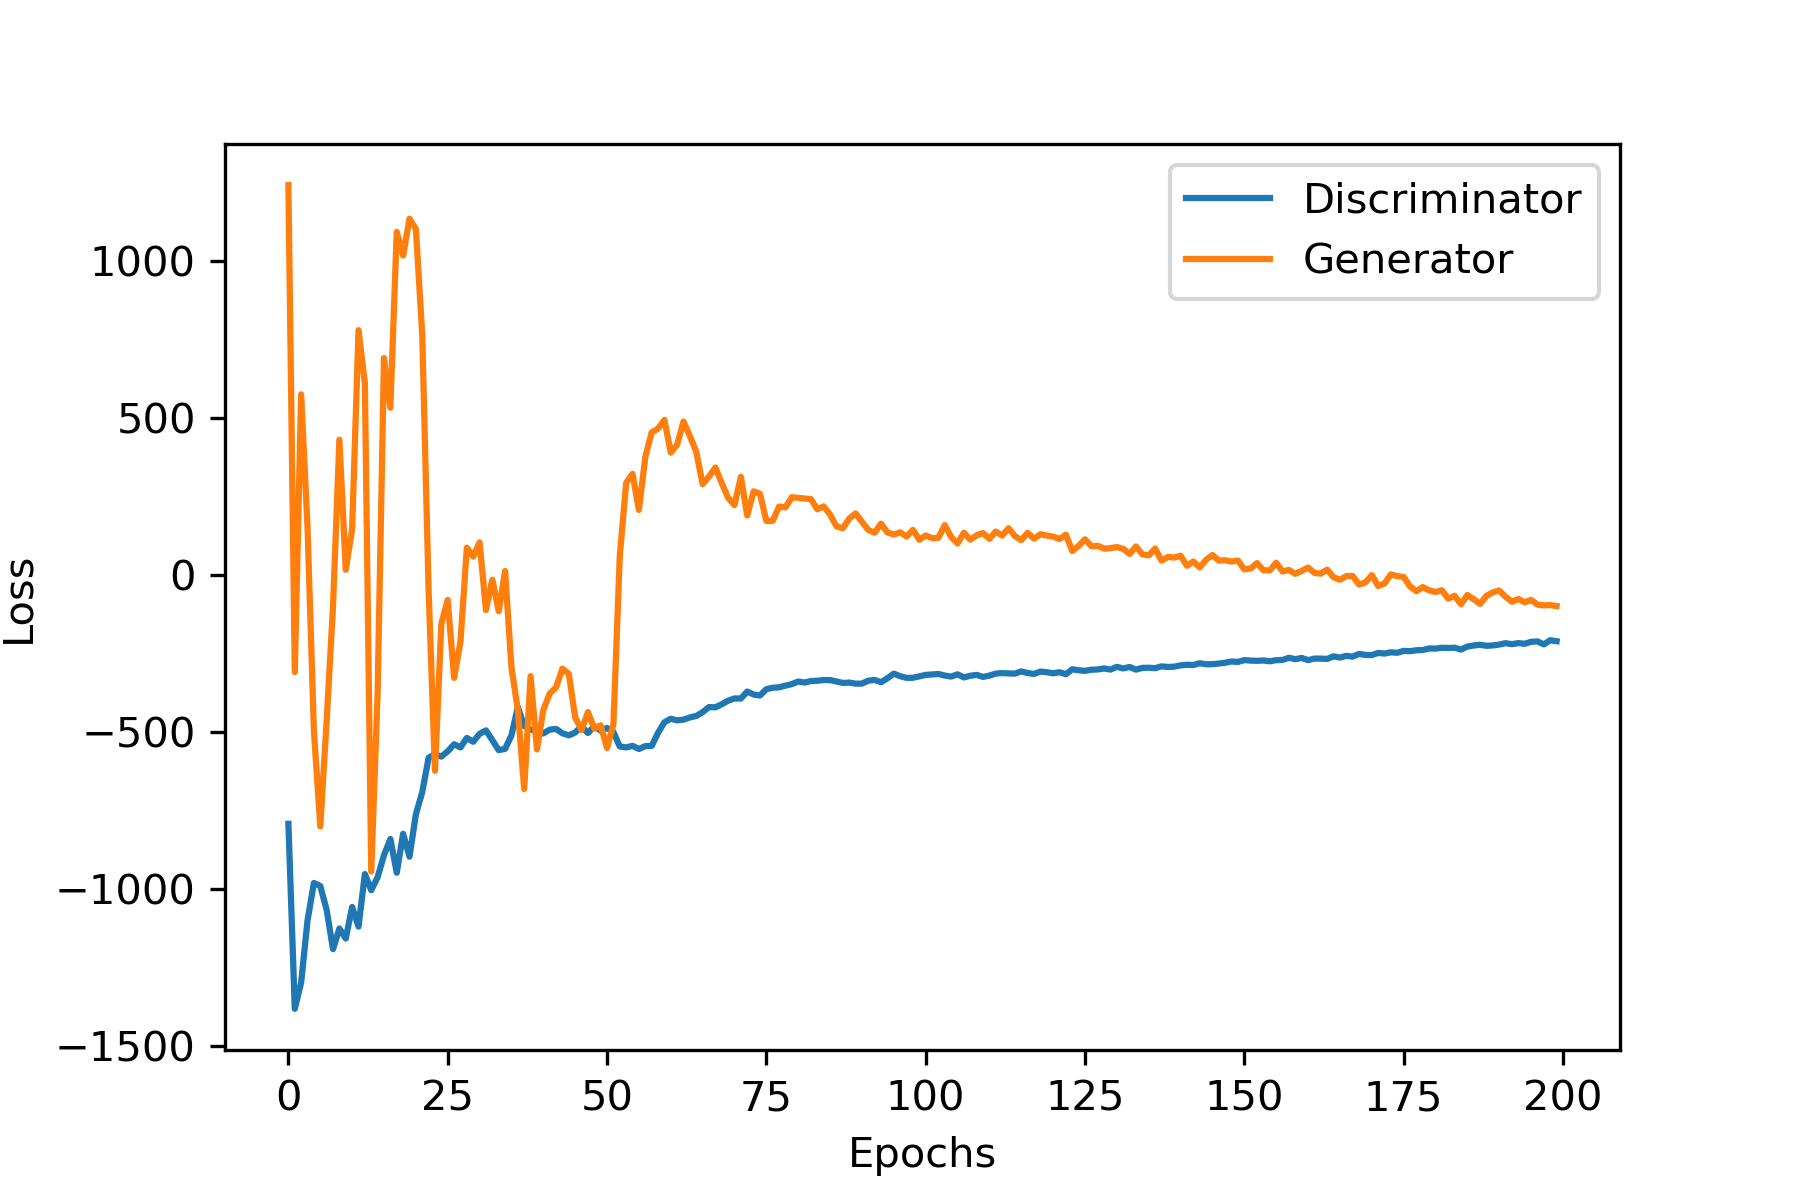
\includegraphics[width=0.48\textwidth]{0725_flute_wpgan_loss.png}
\caption{Left: typical discriminator/generator loss graphs for the naive (strong-topology) GAN. Right: typical discriminator/generator loss graphs for the WGAN-GP.}
\end{figure}\label{dcgan_wpgan}

\subsection{Single Pitch Flute Experiments}
\label{sec:single_pitch_experiments}
In this set of experiments, the GAN architecture was modified using the methods outlined in section \ref{sec:variation} through iterative experiments. During an informal evaluation of the results produced using all flute samples, we noted that it sounded like the generator was trying to produce musical scales or play multiple pitch values at once. Because this dataset contained a wide range different pitches, we hypothesized that this was forcing the generator to learn to pitch of the sound in addition to the timbre of the flute. A decision was made to remove the dimension of pitch and only train using a subset of flute sounds that contained the same pitch. The pitch that contained the most examples was selected. This resulted in a dataset of 177 flute examples playing an F. Each experiment was trained over 1000 epoch using a reduced batch size of 32 to allow the model to be trained on a GPU.

The first set of experiments was focused on the upsampling method in the generator. Five different methods were tested: transpose convolution, upsampling layer, nearest neighbor interpolation, linear interpolation, and cubic interpolation. Out of these methods linear interpolation and cubic interpolation produced poor results judged by an informal listening evaluation and were discarded for subsequent experiments. Batch normalization was then tested using transpose convolution, upsampling, and nearest neighbour interpolation. Experiments with dropout of 50\% were conducted and showed an impressive improvement in reducing noise. Phase shuffling with $N=2$ and kernel sizes $k \in \{5,15,25\}$ were finally tested. Plots of the result discriminator and generator loss for all experiments are provided in Appendix C.

\subsection{Instrument Experiments}
Based on the findings from the single pitch flute experiments, which were evaluated using a combination of nearest neighbour evaluation (described in section \ref{sec:nearest_evaluation}) and an informal subjective evaluation, a model architecture was selected for further training. The selected model used nearest neighbour interpolation, batch normalization, and a drop out of 50\% in the generator, and a kernel size of 25 in the discriminator. Using this, five new generators were trained on flute, guitar, mallet, synth bass, and vocal samples from the NSynth dataset. Single pitches were again selected for each of the datasets, and the pitch that contained a relatively large number of samples within each dataset was selected to maximize the number of samples for each set. Table \ref{tab:single_inst} provides an overview of each of these datasets.

\begin{table}[t]
    \caption{Single Pitch Instrument Training Datasets}
    \label{tab:single_inst}
    \centering
    \begin{tabular}{llll}
        \toprule
        Instrument& MIDI Note& Pitch& Num Samples\\
        \midrule
        Flute&      77&     F5&     177\\
        Guitar&     68&     G\#4&   372\\
        Mallet&     67&     G4&     355\\
        Synth Bass& 39&     D\#2&   660\\
        Vocal&      61&     C\#4&   190\\
        \bottomrule
    \end{tabular}

\end{table}



Each of the flute and mallet GANs were trained for 4000 epochs using a batch size of 32, and then due to limitations on training time, the remaining models were trained for 2000 epochs using a batch size of 32.

\subsection{MelGAN}
A number of experiments were performed using the MelGAN model described in section \ref{sec:methods_melgan}. The single pitch flute dataset that was used in the previous experiments was converted to mel-spectrograms. Two model architectures informed from the time-domain experiments conducted in section \ref{sec:single_pitch_experiments} were selected for experimentation here: transposed convolution layers vs. nearest neighbour interpolation layers, both tested with a dropout of 50\%. Figure \ref{fig:melgan} shows a spectrogram from the training dataset and two spectrograms produced by MelGAN with nearest neighbour interpolation. These results show that the structure of the harmonics was learned quite well in the first example, although misses some of a nuance of the sound. Although checkerboard artifacts aren't visible, listening to the results reveal a noticeable and unpleasant amplitude modulation, most likely due to subtle periodic artifacts from the convolution. The timbre of the sound was represented surprisingly well, but unfortunately due to the severity of the amplitude modulation artifacts the results would not be usable. The second example, on the right, shows a large 'blob' of noise that was produced unexpectedly, again rendering this model unusable.

\begin{figure}
\centering
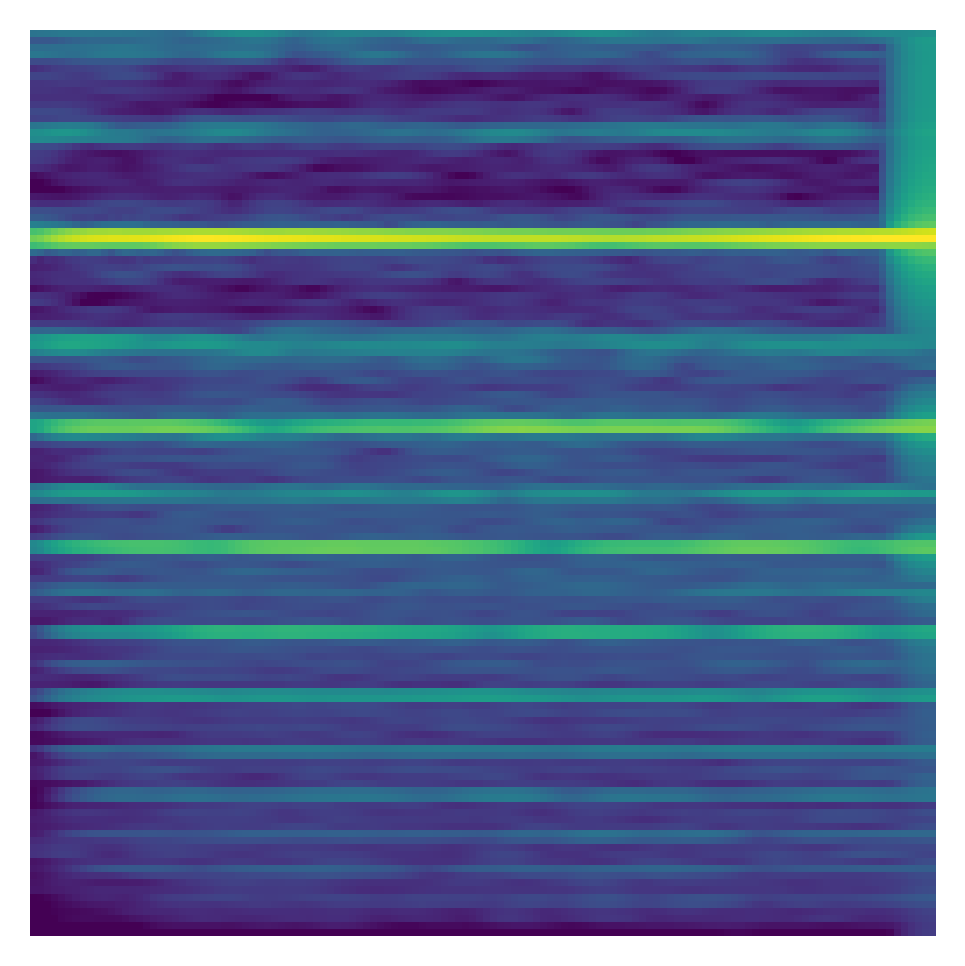
\includegraphics[width=0.32\textwidth]{MelGAN_Train.png}
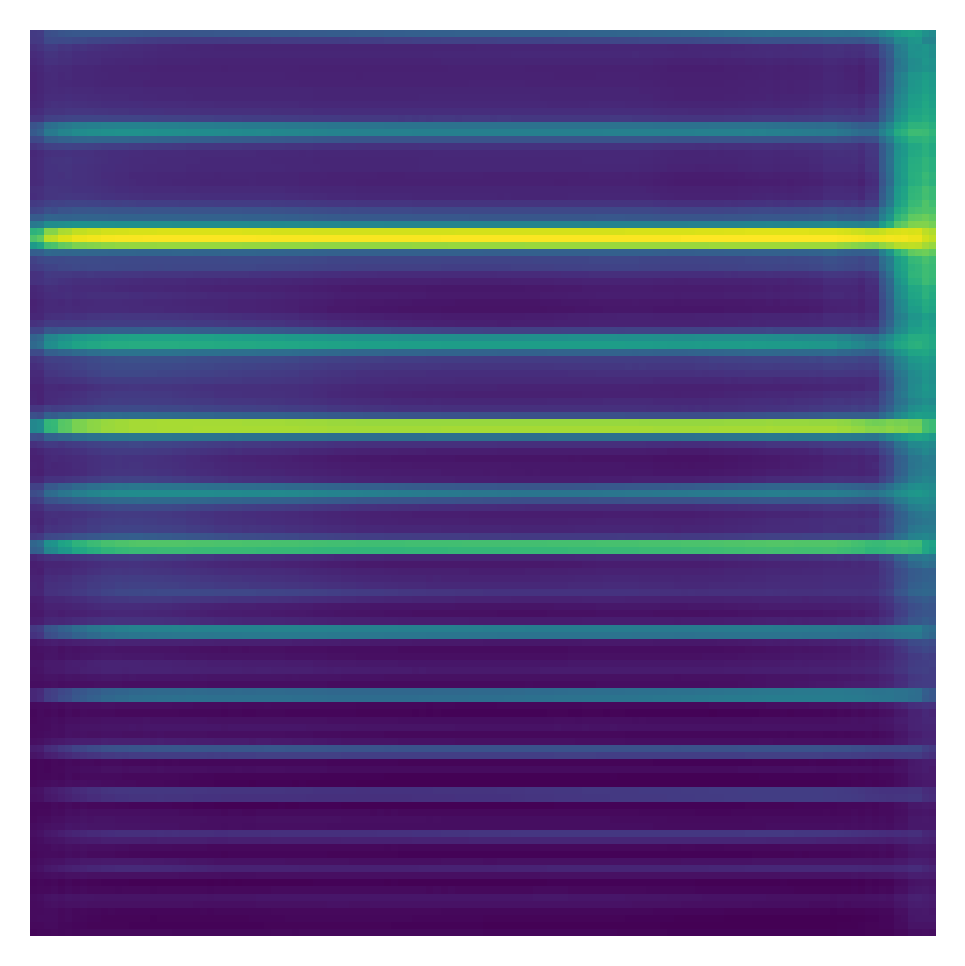
\includegraphics[width=0.32\textwidth]{MelGAN_Generated.png}
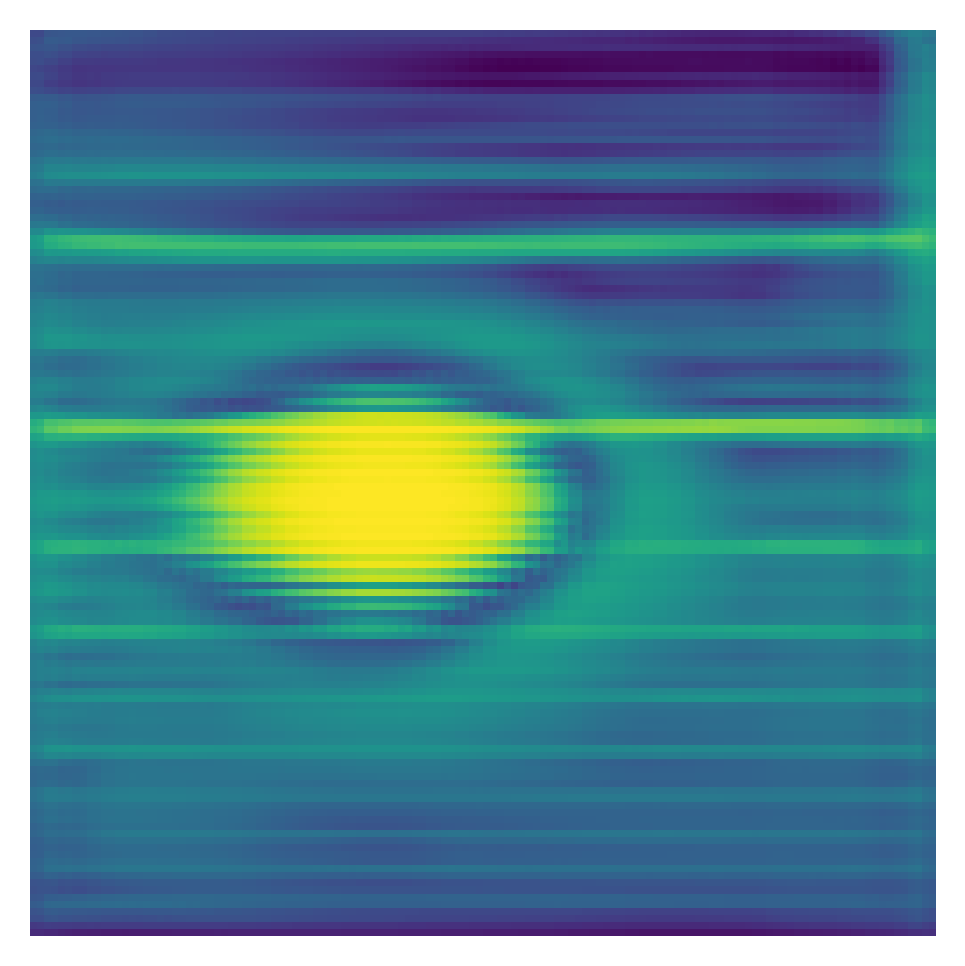
\includegraphics[width=0.32\textwidth]{MelGAN_Blob.png}
\caption{Left: Mel-Spectrogram of flute from the training set. Center and Right: Mel-Spectrograms generated by MelGAN using nearest neighbour interpolation.}
\label{fig:melgan}
\end{figure}

\subsection{Nearest Neighbour Evaluation}\label{sec:nearest_evaluation}
Nearest neighbour is an objective evaluation method proposed by \cite{donahue2018adversarial} and comprises two metrics: $|D|_{self}$ and $|D|_{train}$. $|D|_{self}$ is calculated on a set of samples and is calculated by taking the average Euclidian distance between each sample and its nearest neighbour (excluding itself). This metric provides a measurement of how much variance there is within a dataset. Smaller values of $|D|_{self}$ indicates less variance, and a value of 0 for a generator means that the generator is just producing the same result regardless of the latent input. $|D|_{train}$ is calculated by measuring the average Euclidian distance between every sample in a set of generated samples and its nearest neighbour in the dataset used for training. $|D|_{train}$ provides a measurement of how similar a set of generated samples is to the training dataset, and both measurements together provide insight into how close a generator is getting to the training dataset and the amount of variety the generator is able to learn.

Because time domain audio signals do not provide a measurement that is representative of human perception, 20 Mel-Frequency Cepstral Coefficients (MFCCs) are extracted from each signal and summarized over time using the mean.

\subsubsection{Single Pitch Flute Evaluation}
Evaluation of the models generated from experiments conducted using the single pitch flute dataset (Section \ref{sec:single_pitch_experiments}) was performed by generating 200 random audio samples from each trained model. This resulted in 14 different generated datasets that were evaluated using the two nearest neighbour metrics. The flute training dataset was included in the $|D|_{self}$ measurement. These results are shown in figure \ref{fig:single_pitch_nn}. 

The $|D|_{self}$ results confirm that both linear and cubic interpolation produced results that were not close to the training dataset, and that nearest neighbour interpolation performed the best out of all the resize methods. Adding dropout to the generator had a significant effect on improving the generator's ability to learn the distribution of the flute dataset. Interestingly, increasing the kernel size did not have a hugely significant effect on the learning once dropout had been added. Another interesting result is that several of the models actually produced results that had both greater variance than the training dataset while also having a small value 

\begin{figure}[htbp]
\centering
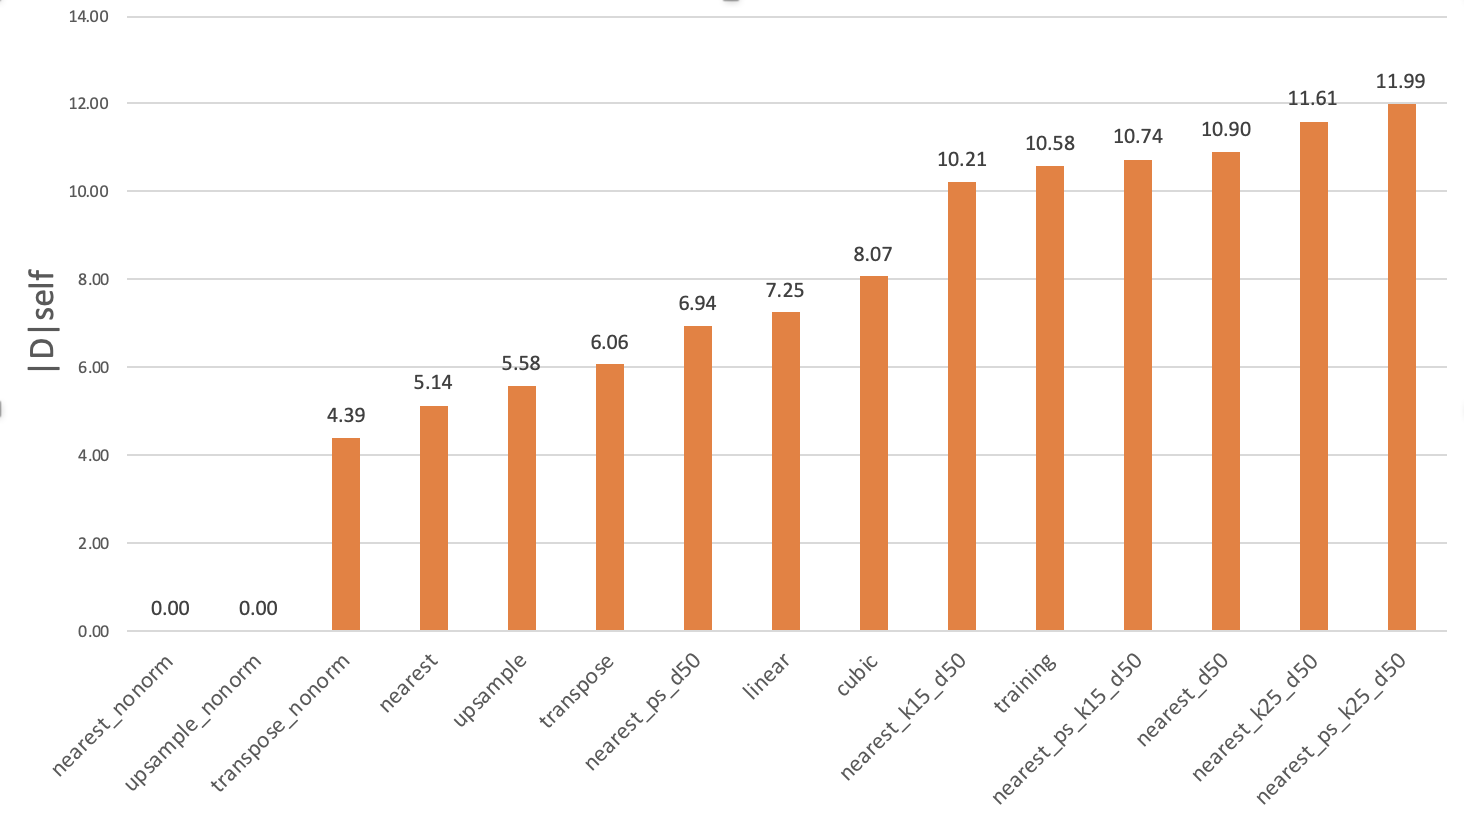
\includegraphics[width=0.75\textwidth]{D_self.png}
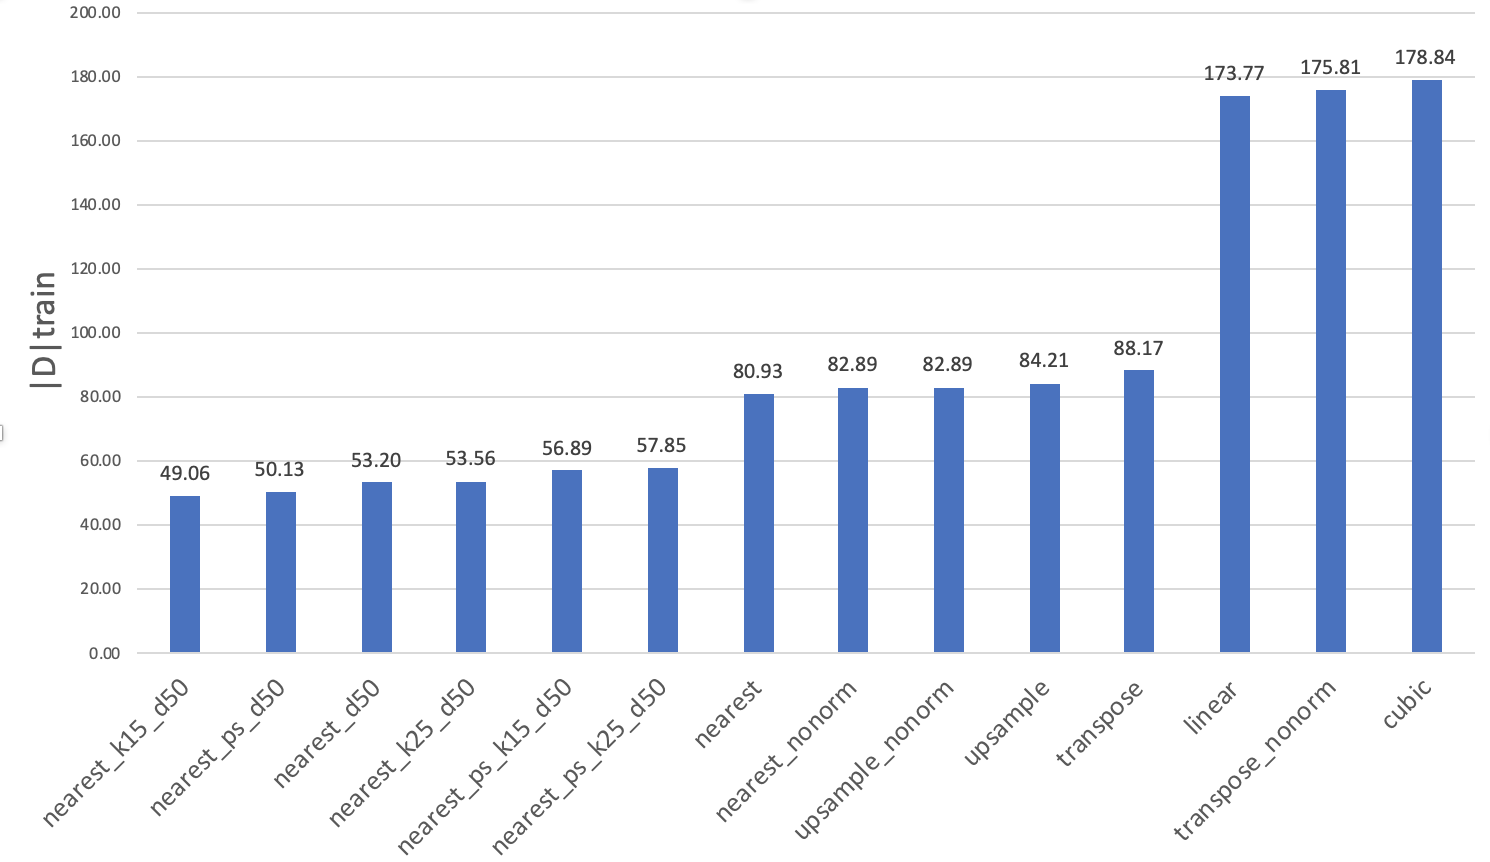
\includegraphics[width=0.75\textwidth]{D_train.png}
\caption{Nearest neighbour evaluation for the single pitch flute experiments. Top: $|D|_{self}$ . Bottom $|D|_{train}$. The model type is indicated in the x-axis by a string giving the upsampling method and then appending any additional changes, where nonorm indicates no batch normalization in the generator, ps indicates phase shuffling in the discriminator, k$n$ indicates the kernel size in the discriminator where $n$ is the kernel size, if no k is provided then the kernel size is 5, and d50 indicates that dropout of 50\% was used in the generator.}
\label{fig:single_pitch_nn}
\end{figure}

\subsubsection{Single Pitch Instrument Evaluation}
Evaluation of the models generated from training the different instrument datasets was performed by generating 500 random audio samples from each trained model: flute, guitar, mallet, synth bass, and vocal. Each of these generated datasets were evaluated using the two nearest neighbour metrics. The datasets used to train each of the models is included in the $|D|_{self}$ metrics. These results are shown in figure \ref{fig:instrument_nn}. Results of $|D|_{train}$ show that the other instrument datasets had more variance between samples than those of the flute dataset, and that the models trained from the datasets did not have the same degree of variance between samples. The results of $|D|_{self}$ are comparable for all training datasets, the mallet generator was closest to the training dataset and the synth bass was most dissimilar.

\begin{figure}[htpb]
\centering
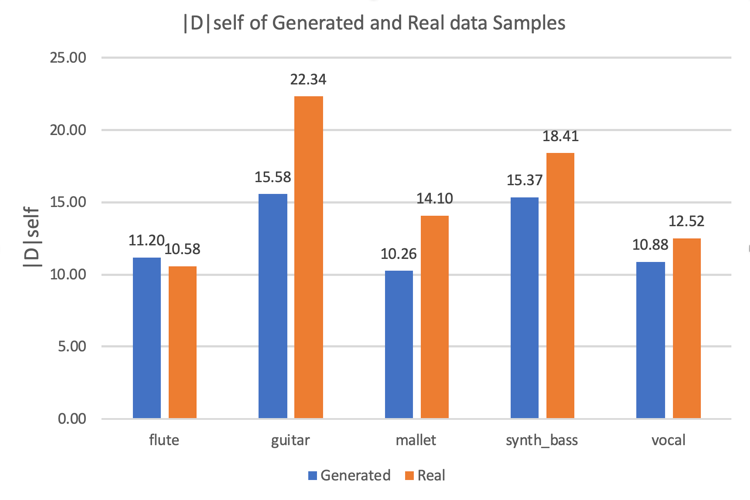
\includegraphics[width=0.49\textwidth]{D_self_gen_real_2.png}
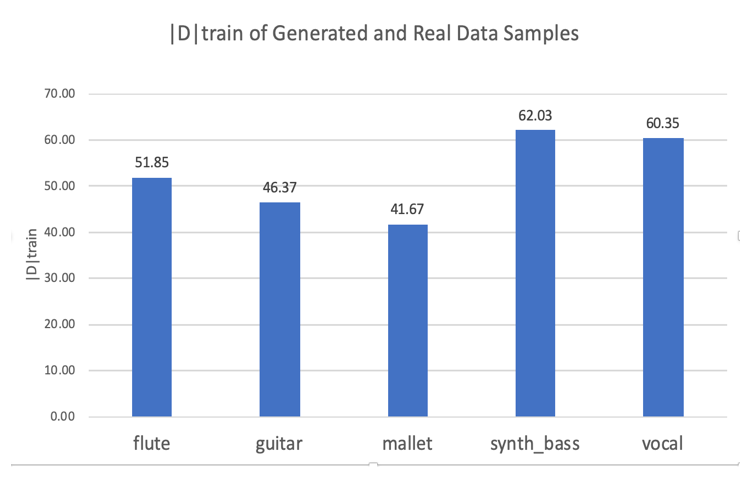
\includegraphics[width=0.49\textwidth]{D_train_gen_real_2.png}
\caption{Nearest neighbour evaluation for the instrument experiments. Top: $|D|_{self}$ . Bottom $|D|_{train}$.}
\label{fig:instrument_nn}
\end{figure}

%\subsection{Qualitative Results}
%Show some plots of the waveform learning, perhaps show some error cases (like the weird hole in the Mel-Spectrogram). PCA plot of the flute learning.

\section{Discussion and Conclusion}

Audio generation in GANs is a relatively unexplored field, especially considered to the sister field of image generation. Our results have been promising, but far from complete. The generated samples have been far from passing any sort of subjective-evaluation Turing tests; however, our generated samples do capture certain key components of the instrument. Both veins of GAN we tried (time-series based and mel-frequency based) exhibited positive and negative features which were in some sense complementary from the other.

The time-series based WaveGAN-like networks were able to generate sounds which were structurally similar to the originals, except that they failed to capture high frequency components of the signal. This could be an effect of the reduced sample rate, or due to the resizing methods we explored. While transpose convolutions are more likely to produce aliasing and noise related to checkerboard artifacts, \cite{donahue2018adversarial} note that these transpose convolution layers may be important in generating high-frequency detail.

The mel-spectrogram-based approach, on the other hand, captured the timbre of the sound fairly well. However, it suffered from the opposite problem as the time-series based networks: structurally, the samples were off, carrying unnatural ``fluttering'' artifacts. These artifacts could be related to ``bump'' artifacts we noticed in the center of some training samples' spectrograms. It is a little puzzling that the discriminator was not able to catch and prevent these artifacts. However, it is rather encouraging that this may be is the stumbling block on which the MelGAN failed. For, preventing these artifacts is a clearly-defined problem in the realm of image generation. It is therefore possible to bring the full brunt of image-based GAN technology to bear on the problem. Furthermore, checkerboard artifacts may be involved, creating strange discontinuities in the spectrum and overemphasizing certain spectral bands.

The resize/upsampling-based approaches were moderately successful in eliminating these checkerboard artifacts. Only nearest-neighbor-style resizing as able to train well;  the generators equipped with either cubic or linear interpolation struggled to improve over time. This agrees with observations made in \cite{Odena2016DeconvolutionAC}: the current state-of-the-art hyperparameters are tuned to efficiently train transpose convolution based generators, which are analogous to nearest-neighbor upsampling based generators. Odena et al. hypothesized that better results may be obtained after a careful search of hyperparameter space aimed at improving cubic interpolation based generators. This is an exciting research avenue which may well yield tremendous improvements in sound quality.

By far, the greatest improvement in sound quality came as a result of adding dropout layers to the neural network. Previously, the networks had only been generating very grating ``rusty doorhinge'' sounds. Dropout layers significantly regularized the samples and made them palatable to the human ear. Because dropout layers are resistant to overtraining, it is possible that training the networks for even longer while using dropout layers would yield improved results.

Because we were only considering the first second of the 4-second-long NSynth samples, it was not possible in general for the GAN to interact with the entire envelope of the samples (except for samples with fast decay, such as the mallet sounds). Our results were therefore generally limited to capturing the samples' attack and timbre. These two properties, however, largely dominate the quality and recognizably of a sound.

One philosophical observation is that in an ideal world, machine learning specialists are able to bring their human intuitions about the structure of a problem to bear on the network architecture. This partially explains the tremendous success of convolutional neural networks in image-related problems: convolution captures salient properties of images, namely spacial proximity and approximate translation-invariance of features (for example the first layer of a CNN tends to capture different types of lines in an image, which are clearly invariant of position on the image).

It is interesting to ponder whether or not the DCGAN architecture captures the relevant features in sound generation. The approach in \cite{donahue2018adversarial}, and in our own work, was to transport successes in image generation with minimal alteration into the field of audio generation. It may be that this is a case of square pegs and round holes.

For example, it is not obvious a priori that convolution in one dimension even `sees' timbre: after all, adjacency in `physical space' is very different from adjacency in spectral space, while spectral space is arguably what we are really noticing when we listen to audio.

The MelGAN has direct access to the spectrum of a sound, and therefore locality on the spectrogram is a reasonable thing to assume. However, the translational invariance property of CNNs is a reasonable thing to question in this context. For, while translation in the x-axis corresponds to translation in time, which is a very reasonable thing to assume translation invariance for, vertical translation is a different beast. For, the scaling of frequency bands (whether linear, logarithmic, or other) now becomes a crucial point. What is to say that ``a straight line'' in the upper frequencies of a spectrogram in any way corresponds to a straight line in the lower frequencies, especially if the straight line is not horizontal? It may be profitable to treat a spectrogram less as an image and more as a time-series of spectral coefficient vectors, perhaps by prioritizing the y axis in the network architectures.

This paper has only brushed the tip of the problem of audio generation, but even this short exploration has illuminated a vast spectrum of audio-related challenges and promising avenues for possible research.